



\documentclass[11pt, a4paper]{article}

%MUST DOWNLOAD algorithm.sty
\usepackage{algorithm} 
%\usepackage{algorithmicx}
\usepackage{algpseudocode}
\usepackage{empheq}
\usepackage{euscript}
\usepackage{amsmath}
\usepackage{amsthm}
\usepackage{amssymb}
\usepackage{epsfig}
\usepackage{xspace}
\usepackage{color}
\usepackage{url}
\usepackage{hyperref}
%\usepackage{algpseudocode}

\usepackage{mathtools}
\DeclarePairedDelimiter\ceil{\lceil}{\rceil}
\DeclarePairedDelimiter\floor{\lfloor}{\rfloor}

%%%%%%%  For drawing trees  %%%%%%%%%
\usepackage{tikz}
\usetikzlibrary{calc, shapes, backgrounds}

%%%%%%%%%%%%%%%%%%%%%%%%%%%%%%%%%
\setlength{\textheight}{9in}
\setlength{\topmargin}{-0.600in}
\setlength{\headheight}{0.1in}
\setlength{\headsep}{0.250in}
\setlength{\footskip}{0.4in}
\flushbottom
\setlength{\textwidth}{6.5in}
\setlength{\oddsidemargin}{0in}
\setlength{\evensidemargin}{0in}
\setlength{\columnsep}{2pc}
\setlength{\parindent}{1em}
\setlength\fboxsep{1cm}
%%%%%%%%%%%%%%%%%%%%%%%%%%%%%%%%%


\newcommand{\eps}{\varepsilon}

\renewcommand{\c}[1]{\ensuremath{\EuScript{#1}}}
\renewcommand{\b}[1]{\ensuremath{\mathbb{#1}}}
\newcommand{\s}[1]{\textsf{#1}}
\newcommand*\widefbox[1]{\fbox{\hspace{2em}#1\hspace{2em}}}
\newcommand{\E}{\textbf{\textsf{E}}}
\renewcommand{\Pr}{\textbf{\textsf{Pr}}}
%
% enumerate labeling paradigm. Below is alphabetical
%
%\renewcommand{\labelenumi}{(\alph{enumi}) }



%%%
%%%  Header
%%%


\begin{document}
\begin{center}
    {\Large Classification of Songs via Homology of Chroma Features}\\
   Computational Topology \hfill CS6170\\
  Zahra Fahimfar \hfill uNID: u0900547\\
  Samuel Leventhal\hfill  uNID: u0491567
\end{center}
%%%%%%%%%%%%%%%%%%%%%%%%%%%%%%%%%%%%%%%%%%%%%%%%%%%%%%%
%%%%%%%%%%%%%%%%%%%%%%%%%%%%%%%%%%%%%%%%%%%%%%%%%%%%%%%
%%%%                                              %%%%%
%%%%       Reference of Latex functionalities     %%%%%
%%%%                                              %%%%%
%%%%%%%%%%%%%%%%%%%%%%%%%%%%%%%%%%%%%%%%%%%%%%%%%%%%%%%
%%%%%%%%%%%%%%%%%%%%%%%%%%%%%%%%%%%%%%%%%%%%%%%%%%%%%%%
\iffalse
%
% Image
%
\begin{figure}[H]
\centering{
\includegraphics[width=.8\linewidth]{problem1plot.png}
}
\label{fig:prob1fig}
\end{figure}

%
% Matrix
%
\[ \begin{pmatrix}
  4 & 1 \\
  0 & 4 \\
\end{pmatrix}\]

%
% Algorithm
%
  \begin{algorithm}[H]
\caption{Matrix Inversion by LU decomposition}
\begin{algorithmic}
  \For{$k = 1:n$}
      \For{$i=1:n$}
          \If{$i\neq k$}
              \State $l_{ik} \leftarrow \frac{A_{ik}}{A_{kk}}$ \Comment{(n-1)}
                    \For{$j=k+1 : 2n$}
                        \State $A_{ij} \leftarrow A_{ij} - l_{ik}A_{kj}$ \Comment{2(n-1)(2n-k)}
                    \EndFor
                    \EndIf
                    \For{$j=2n:k$}
                    \State $A_{kj} \leftarrow \frac{A_{kj}}{A_{kk}}$ \Comment{2n-k+1}
                    \EndFor
      \EndFor
  \EndFor
\end{algorithmic}
\end{algorithm}

%
% Another matrix
%
  \[
  \begin{smallmatrix}
    1 & 1 & 1 & \cdots & 1 & 2 & 3 & 4 & \cdots & n & 2 & 3 & \cdots &n\\
    1 & 2 & 3 & \cdots & n & 1 & 1 & 1 & \cdots & 1 & 2 & 3 & \cdots & n\\
    c_{1,1} & c_{1,2} & c_{1,3} & \cdots & c_{1,n} & c_{2,1} & c_{3,1} & c_{4,1} & \cdots & c_{n,1} & c_{2,2} & c_33 &\cdots &c_nn\\
  \end{smallmatrix}
\]

%
% bounding box
%
\noindent\fbox{
  \parbox{.8\textwidth}{

  }
}



\fi
%%%%%%%%%%%%%%%%%%%%%%%%%%%%%%%%%%%%%%%%%%%%%%%%%%%%%%%%%%%%%%%%%%%%%%%%%
%%%%%%%%%%%%%%%%%%%%%%%%%%%%%%%%%%%%%%%%%%%%%%%%%%%%%%%%%%%%%%%%%%%%%%%%%
%%%%%%%%%%%%%%%%%%%%%%%%%%%%%%%%%%%%%%%%%%%%%%%%%%%%%%%%%%%%%%%%%%%%%%%%%
\begin{enumerate}
  
\item \textbf{  Project overview}
  
  Most common in learning algorithms for music is to classify songs based on user input, where song labels are determined by a user's cluster of preferred music. We aim to instead label songs based on structural similarities. Specifically, we aim to classify songs based on topological similarities after embedding a song's musical composition in euclidean space using the pitches and their time signatures within the composition.

\item \textbf{Motivation \& Merit}

  Most of the current methods for song recommendation are based on the song similarity among users' common songs. This is called collaborative filtering recommendation. This project attempts to propose a content based filtering recommendation method where similar songs are found based on their inner content and structure, rather than the users who have listened to them. Therefore, the proposed method is completely independent of clustering of songs based on user groups or ``genre'', instead, song similarities are extracted from their implicit compositions and structures. A topologically based learning algorithm as proposed here allows new means of studying music theory and novel approach to music classification and recommendation. 

  \item \textbf{Technical details}
    \begin{itemize}
    \item \textbf{Methodology:}
      Our goal is to represent musical data in a form which allows us to extrapolate topological attributes unique to each song. These topological attributes, be it homologies or manifold structures, would then afford features to construct a novel means of song classification. 
      
      $\ \ \ \ $ Our approach will then first \textbf{(1)} construct a data structure based on song data such as an associated matrix with weights or a point cloud in euclidean space followed by \textbf{(2)} using persistent homology or manifold modeling to extrapolate features to be used in \textbf{(3)} a machine learning approach to classify musical compositions as similar.

    \item \textbf{Data:}
      Using the Million Song Database  we aim to extrapolate key musical structures identified topologically to be used as features for label classification of music by genre. Features of interest are
      \begin{itemize}
          \item \textit{Fugue Attributes:} Subjects, Countour Subjects, Sequences, Cadences, and Structure.
          \item \textit{Variations:} Fragmentations, Parallelism, and Theme Reduction
          \item \textit{Texture:} Model of Texture, and Homorhythmic Layers.
          \item \textit{Chroma Features:} In music audio for each time step a note or group of notes are played composing a single tone. In total there are 12 fundemental tones which can be translated by octave to form an equivilance class. Similar to modular arithmatic the entire spectrum of tones can be seen as a group generated by 12 distinct semitones, or chroma. Chroma features allow a powerful representation of music audio by expressing the fundemental structural form of the original spectra. Chroma Feature Analysis: \url{https://labrosa.ee.columbia.edu/matlab/chroma-ansyn/}
          \item \textit{Audio Files:} .OGG or .WAV
      \end{itemize}

    \item \textbf{Normalization:}
      Normilisation of the data affords a means of preventing minor deviations in the data in the data in terms of signifigance which may produce topologically significant structures. 
      
    \item \textbf{Datasets:}
      \begin{itemize}
      \item \textit{pitch and timing:} OGG files, Scores on IMSLP, \textbf{ Million Song Dataset} (\url{https://labrosa.ee.columbia.edu/millionsong/}) for metadata features and 7digital (\url{ http://www.7digital.com/}) for sample audio of songs. Also available is \textbf{Polyphonic Melody Extraction} \url{https://labrosa.ee.columbia.edu/projects/melody/} 
      \item \textit{Fugue} \url{http://algomus.fr/datasets/fugues.truth.2013.12}
      \item \textit{texture:} \url{http://algomus.fr/datasets/texture.truth.2014.10}
      \item \textit{genre:} Million Song Dataset and 7digital for sample audio of songs using code (\url{https://github.com/tb2332/MSongsDB/tree/master/Tasks_Demos/Preview7digital}) provided by Million Song Dataset.
        \item \textit{IMSLP} all public domain music \url{http://imslp.org/}
        \item All metadate features listed also available through Audio Content Analysis \url{http://www.audiocontentanalysis.org/data-sets/}
      \end{itemize}

      
  \item \textbf{Data Structure:}
    \begin{itemize}
    \item \textit{Graph Representation:}  Each node corresponds to a pitch occurring in a musical piece along with the starting and stopping time of that pitch, specifically\\ $ \{ pitch, (t_{start(pitch)}, t_{stop(pitch)}) \} $. Edges of the graph correspond to nodes which are sequential. Each edge then correlates to pitches within a song which are consecutive. Weights could also be added to edges and valued proportional to the number of occurred sequential pairing. The larger the edge weight the more common than a series of pitches is.

    \item \textit{Matrix Construction:} Element $t_{i,j}$ of matrix $T$ implies pitch $i$ occurs before and is directly followed by pitch $j$. The rows and columns of $T$ correspond to observed pitches within the song. Element $t_{ij}$ contains the start and stop times of the consecutive pitches $i$ and $j$ as they have occurred throughout the song, specifically $\{[ (t^1_{start(i)}, t^1_{stop(i)}), \cdots ,t^m_{start(i)}, t^m_{stop(i)})]  , [(t^1_{start(j)}, , \cdots , t^m_{stop(j)})] \}$ and imply pitch identified to row $i$ occurs at $t^{\ell}_{start(i)}$ and lasts for  $ t^{\ell}_{stop(i)} - t^{\ell}_{start(i)}$ for each $\ell$ such that $1\leq \ell \leq m$ where $m$ is the total number of times pitch $i$ precedes pitch $j$ identified with column $j$ and beginning at $t^{\ell}_{start(j)}$ and lasting for $t^{\ell}_{stop(j)} - t^{\ell}_{start(j)}$.

    \item \textit{Coordinate Mapping:} Two options are available for a coordinate representation. The first would be to take the matrix representation discussed above and translating it into a graphical representation. The second would be to plot each pitch directly into $\mathbb{R}^3$ where the coordinate $(x,y,z)$ is defined to be $(start\ time, stop\ time, pitch)$. Embedding each song in euclidean space in this manner allows each song to be represented as a point cloud in $\mathbb{R}^3$ consisting of every pitch that occurs in a song. 
    \end{itemize}

    
  \item \textbf{Topological data analysis techniques:}
    
    \begin{itemize}
    \item \textit{Persistent Homology:} Taking advantage of having each song represented as a point cloud persistent homology will allow us to identify the birth and death homological features unique to a musical composition. The dimension and quantity of homological features along with their birth and death times during persistence can then serve as musical compositions ``finger print''. This finger print, consisting of what homological features emerge and when, during persistence, they are born and die will allow us a means to relate separate songs.

      $\ \ \ \ $Regardless of whether we choose to use a matrix representation which is then translated into a point cloud or directly plot our data as a point cloud the use of persistent homology will achieve the same goal. Persistent homology will allow us to extrapolate recurrent musical structures dependent on the scale, with respect to the filtration used in persistent homology, these features are born and die. If we are to consider our data as pitch, time of being played, and stop time persistence will allow us to relate homological features based on musical composition. We suspect these homological features will correlate to melodies and chord compositions shared between songs. We suspect this because similar homological features will be born and die at similar times in different songs if both those songs contain common patterns of pitch/time signatures. For example, figure \ref{fig:persMusic} demonstrates two a repeated sequence of pitches which repeats at $t$ and $t^*$ and two different stages of persistence shown in red and blue. From the two stages of persistence shown in figure \ref{fig:persMusic} we can see that the time with respect to persistence and the dimension homological features are born and die will be dependent on the composition of the song. For example two songs may share the dimension 1 homological feature formed by the simplicial complex in red. This would imply these two songs both have pitches similar to $p_1$, $p_2$, and $p_3$ which occur sequentially with similar time signatures. The dimension, birth time, and death time of these homological features found during persistence will then serve as a robust feature representation of the musical composition of each song, allowing us to apply various machine learning techniques to label various musical pieces as similar.

      \begin{figure}[H]
        \centering
        \label{fig:persMusic}
        \centering{
          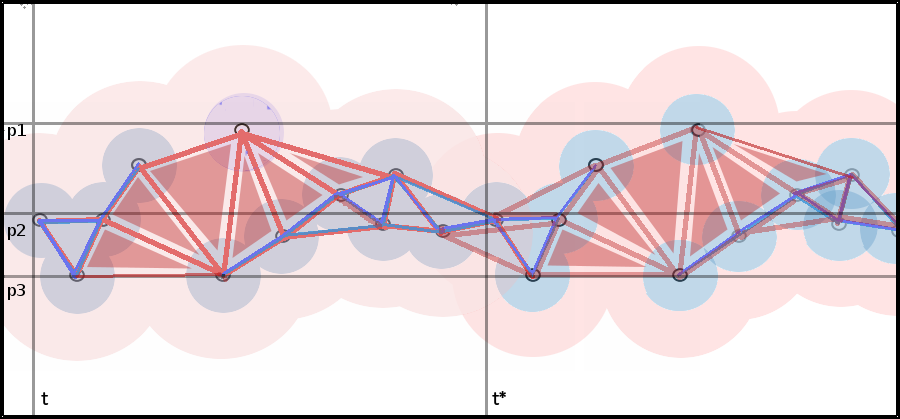
\includegraphics[width=.8\linewidth]{musicPersistence.png}
        }
        \label{fig:persMusic}
        \caption{Two levels of persistence for musical data}
        \label{fig:persMusic}
      \end{figure}

      \textit{Bottleneck \& q-Wasserstein Distance:}

      The persistence diagrams associated to each song allows us the ability to relate songs in terms Bottleneck and q-Wasserstein distances. These metrics demonstrate the distance between the lifespans of homological features found during persistence of the songs songs chromatic structures. Songs near in Bottleneck and q-Wasserstein distances are then expected to me structurally similar in terms of musical composition. 

    \item {\large \textit{Manifold Modeling:}}
   Another option we are considering second to persistent homology would be a manifold modeling approach such as \textit{isomap} which computes piecewise linear approximation to geodesic distance through the construction of a nearest neighbor graph using the metric of some ``ambient space'' that the manifold of musical data is assumed to belongs, allowing us to say the geodesic distances between nearby samples can be accurately approximated by the distances in the ambient space. Using this metric multidimensional scaling on the pairwise approximate geodesic distances yields a distance preserving $d$-dimensional Euclidean configuration of points. Isomap could then provide a discrete mapping $z_i = f(y_i)$ defined only on the original input samples of pitch relation matrices defined as $S_y = \{y_1,\cdots , y_n \} \in \mathcal{A}$.

    $  \ \ \ \ $ The next step would then be to use the parameterization and coordinate mapping $f$ given by isomap for the construction of a generative manifold model. The  song  matrix data  $S_y$ are considered samples from a random variable $Y$ with an arbitrary density $p(y)$ defined on $\mathcal{A}$. We can then consider the coordinate mapping yielded from isomap  $f:\mathcal{A} \rightarrow \mathcal{C}$ as representing a $d-$dimensional parameterization of $\mathcal{A}$ where each point on the manifold represents the average over all song matrices with the same parameter $f(Y)$.  We can then apply a conditional expectation $g(x) = E[Y-f(y) = x])$ to represent an explicit manifold representation. The conditional expectation $g(x)$, estimated by manifold kernel regression, is then summarized as a manifold representation of from the original song data by the operator $\phi (\cdot ) = g\circ f$. In summary we are then  modeling the coordinate mapping $f$ onto the complete ambient space as a kernel regression on the discrete $z_i = f(y_i)$ done in by first (1) computing $S_z = \{ z_1, \cdots , z_n \}$ by isomap on $S_y$ then (2) building the generative manifold model with (a) the coordinate mapping $f$ by the kernel regression over $S_z$ and (b) the explicit manifild representation $g(x) = E[Y-f(Y)=x] $ estimated by manifold kernel regression.
    \end{itemize}
    
    \end{itemize}

  \item {\large \textbf{Predictive Model}}
    Here we will explain the machine learning component used from the TDA results in order to correlate related songs. Thre core methods for labeling songs as similar are used
    \begin{itemize}
    \item {\it K-Means Clustering:} Using the bottleneck distance and the q-Wasserstein distance as our metric between the persistent homology of songs it is possible to cluster songs using the K-means techniques. The motivation for this approach relies on the assumption that songs who have near persistence diagrams necessarily share musical structures which equate to homological features found during persistence.
    \item {\it K-Nearest Neihgbors:} Founded on the same logic as used in K-means clustering the Bottleneck and q-Wasserstein distance afford a metric to emply machine learning clustering algorithms.
    \item {\it Multidimensional Scaling:} Multidimensional scaling allows a method of visualising the similarity between songs based on the Bottleneck between the respective persistence diagrams. Multidimensional scaling allows a non-linear lower dimensional embedding which preserves the bottleneck distance between persistence diagrams of songs. The lower dimensional embedding is obtained by contructing a $n\times n$ for $n$ songs where index $ij$ holds $\delta_{ij} = bottleneck(pers(song_i), pers(song_j))$ which is the Bottleneck distance between persistence diagrams of songs defining row $i$ and row $j$. Multidemensional then outputs a coordinate matrix whose configuration minimizes some loss function based on the Bottleneck distance.
    \end{itemize}
    
    
\item {\large \textbf{Expected Results}}
  \begin{itemize}
  \item \textit{Expected Outcome:}
    We suspect with the use of tools common to computational topology our project will provide a robust frame work to identify key music theoretic features such as meter, harmonic progression, song motifs, substitute chords within a progression, ect... It will then be an easy extension to apply machine learning techniques to build an accurate song/ song attribute classifier. 

    
  \item \textit{Potential Impact:}
    It is unlikely the proposed approach will be time/space efficient in comparison to algorithms used by Spotify or Pandora however our approach will introduce a new means to study and classify musical compositions in a manner that would be beneficial to music producers. For example programs like Abelton Live would benefit greately in being able to identify/predict musical progressions for a user based on their current song composition similar to the t9 functionality which predicting a users sentence while writing a text.

    
      Three future directions this project can be taken are
      \begin{enumerate}
      \item Study persistence of song data and cluster songs into groups of similar persistent homology
      \item Use key components such as chord progressions and other musical ``units'' as a ground truth to compate to observed song structures in order to identify structures in songs.
      \item Use either persistent homology or extrapolated musical structures to label songs by genre based on genre of songs classified as similar in persistence.
      \item Use predictive model to train probabistic musical sequences in order to generate / predict musical progression given subset of musical composition.
      \end{enumerate}


  \end{itemize}
\end{enumerate}

  {\large {\bf Current questions and obsticals during development}}{\small (not to be in final write-up)}
  
  \begin{itemize}
  \item what is the sampling rate used by the database for each song, currently 2 is being used
  \item How do you obtian the song title field from the .h5 file in order to listen to the songs
  \item What is a machine learning technique which can be used to classify songs as similar using bottleneck/q-wasserstein distance
  \item Is there any beneficial use of reeb graph or mapper?
  \item Questions to address in write-up: what space does my data lie in, what is a notion of distance /similarity in that space, what is the shape structure of my data within that space, hoe are key variables of interest distributed across this ``shape'', what toililicical/geometric summaries are usefull. Persistence homology:list of homolofies, Mapper: nerve of data and cluster of nerves.
  \item can we use k-meands or k-nearest neighbors of persistence diagrams in order to cluster? other clustering techniques?
  \item Can we say chroma features are our form of sparcification to extrapolate key homological features?
  \item option for clustering:
    \begin{enumerate}
    \item Find max and minimum bottleneck distances between songs to determine range.
    \item Divide that interval into however many clusters desired
    \item Group all songs whose pairwise distances are within the previously found interval ranges.
    \end{enumerate}
    Available clustering techniques
    \begin{enumerate}
    \item Simple K means
    \item K-Medoid clustering
    \item Multi-Dimensional Scaling
    \item Use mult-dimensional scaling as input for other clustering techniques. 
    \end{enumerate}
  \item Need to identify song names and genre as well as after clustering. We will then listen in comparison as well as, and more importantly, look at which genre's are contained in each cluster as a quality measure of using persistence for clustering audo files.
  \item use only intensties to find keys used in song, use intensities only to findkey and sympathetic frequencies. Have to limit range of pitches.
  \item Problem with chroma features: due to modular nature of chroma features you dont capture inversions because rather than a 1/5th away rather than a 1/4th they still capture sympathetic value but not necessarily equal.
  \item Complete search for similar songs to 12-bar blues
  \item complete clustering and quality measure of overlap with songs listed as similar in h5 file.
  \item make descriptive image of spectogram w/ persistence over it
  \item make description of image of 12 bar blues spectograms/persistence diagrams
  \end{itemize}
  
\end{document}
%%% Local Variables:
%%% mode: latex
%%% TeX-master: t
%%% End:
